\section{Durchführung}
\label{sec:Durchführung}

\subsection{Messung bis 1 bar}

Zur Aufnahme der Dampfdruckkruve im Druckbereich  $p \leq \qty{1}{bar}$ wird die 
in Abbildung \ref{fig:tiefdruck} zu sehende Messapparatur verwendet. 
\begin{figure} [H]
    \centering
    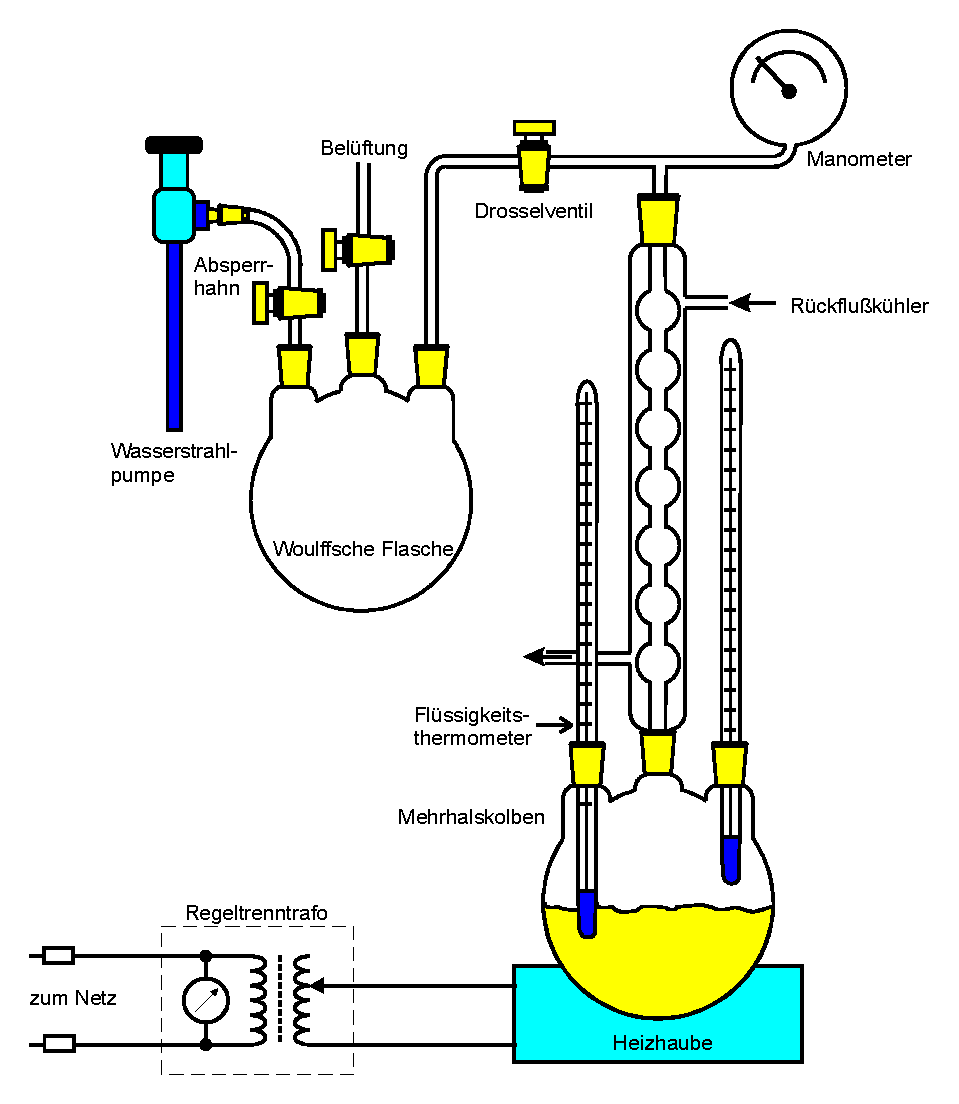
\includegraphics[width=12cm] {pictures/tiefdruck.pdf} 
    \caption{Aufbau der Messapparatur für den Druckbereich $p \leq \qty{1}{bar}$. \cite[6]{v203}}
    \label{fig:tiefdruck}
\end{figure} 

Zu Beginn wird der Umgebungsdruck gemessen, bevor die Apparatur evakuiert wird.
Hierzu müssen der Absperrhahn und das Drosselventil geöffnet und das Belüftungsventil geschlossen werden.
Die Wasserstrahlpumpe wird angestellt, bis sich ein konstanter Druck einstellt. 
Sobald sich der Druck eingestellt hat, 
werden der Absperrhahn und das Drosselventil geschlossen und die Wasserstrahlpumpe abgestellt.
Anschließend wird die Wasserkühlung angestellt, um den aufsteigenden Dampf wieder zu kondensieren. 
Die Heizhaube wird angestellt, um die Flüssigkeit im Mehrhalskolben zu erhitzen. 
Während des Erhitzungsvorgangs wird die Kühlung immer wieder verringert. 
Die Temperatur und der zugehörige Druck werden konstant am Thermometer im Gasraum beziehungsweise am Manometer abgelesen. 
Die Datenpaare werden bei allen ganzzahligen Temperaturen notiert. 
Diese Messung wird durchgeführt, bis der Umgebungsdruck von $\qty{1}{bar}$ erreicht ist.


\subsection{Messung von 1 bis 15 bar}

Zur Aufnahme der Dampfdruckkruve im Druckbereich $p \in [1, 15] \, \mathrm{bar}$ wird die 
in Abbildung \ref{fig:hochdruck} zu sehende Messapparatur verwendet. 
\begin{figure} [H]
    \centering
    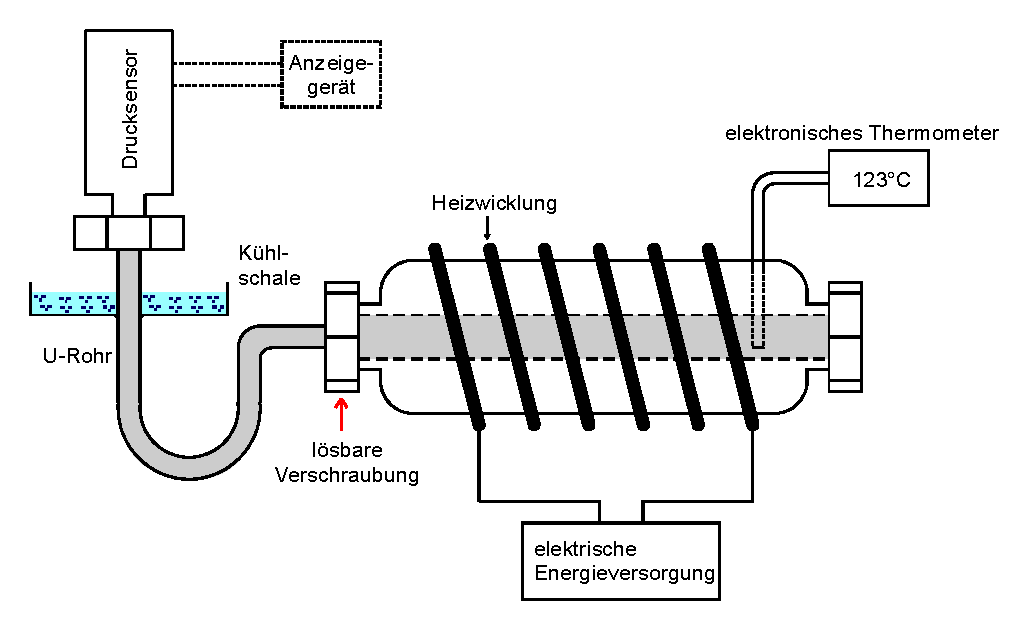
\includegraphics[width=12cm] {pictures/hochdruck.pdf} 
    \caption{Aufbau der Messapparatur für den Druckbereich $p \in [1, 15] \, \mathrm{bar}$. \cite[8]{v203}}
    \label{fig:hochdruck}
\end{figure} 

Die in Abbildung \ref{fig:hochdruck} zu sehende Apparatur ist vor dem Beginn des Versuches bereits mit Wasser gefüllt. 
Allerdings wird bei dieser Messung auf eine Kühlschale verzichtet, da das verwendete Druckmessgerät ausreichend isoliert ist.
Die Heizung wird angestellt und es werden die Datenpaare von Druck und Temperatur pro $\qty{1}{bar}$ notiert. 
Die Messung wird solange durchgeführt, bis $\qty{15}{bar}$ erreicht sind.